% This template has been tested with LLNCS DOCUMENT CLASS -- version 2.20 (24-JUN-2015)

%"runningheads" enables:
%  - page number on page 2 onwards
%  - title/authors on even/odd pages
%This is good for other readers to enable proper archiving among other papers and pointing to
%content. Even if the title page states the title, when printed and stored in a folder, when
%blindly opening the folder, one could hit not the title page, but an arbitrary page. Therefore,
%it is good to have title printed on the pages, too.
\documentclass[runningheads,a4paper]{llncs}[2015/06/24]

\makeatletter
\renewcommand\paragraph{\@startsection{paragraph}{4}{\z@}%
            {-2.5ex\@plus -1ex \@minus -.25ex}%
            {1.25ex \@plus .25ex}%
            {\normalfont\normalsize\bfseries}}
\makeatother
\setcounter{secnumdepth}{2} % how many sectioning levels to assign numbers to
\setcounter{tocdepth}{4}    % how many sectioning levels to show in ToC

%cmap has to be loaded before any font package (such as cfr-lm)
\usepackage{cmap}
\usepackage[T1]{fontenc}

\usepackage{graphicx}
\graphicspath{ {images/} }

%Even though `american`, `english` and `USenglish` are synonyms for babel package (according to https://tex.stackexchange.com/questions/12775/babel-english-american-usenglish), the llncs document class is prepared to avoid the overriding of certain names (such as "Abstract." -> "Abstract" or "Fig." -> "Figure") when using `english`, but not when using the other 2.
%english has to go last to set it as default language
\usepackage[ngerman,english]{babel}
%Hint by http://tex.stackexchange.com/a/321066/9075 -> enable "= as dashes
\addto\extrasenglish{\languageshorthands{ngerman}\useshorthands{"}}

%better font, similar to the default springer font
%cfr-lm is preferred over lmodern. Reasoning at http://tex.stackexchange.com/a/247543/9075
\usepackage[%
rm={oldstyle=false,proportional=true},%
sf={oldstyle=false,proportional=true},%
tt={oldstyle=false,proportional=true,variable=true},%
qt=false%
]{cfr-lm}
%
%if more space is needed, exchange cfr-lm by mathptmx
%\usepackage{mathptmx}

%for demonstration purposes only
\usepackage[math]{blindtext}

%Sorts the citations in the brackets
%It also allows \cite{refa, refb}. Otherwise, the document does not compile.
%  Error message: "White space in argument"
\usepackage{cite}


%% If you need packages for other papers,
%% START COPYING HERE
%% COPY ALSO cmap and fontenc from lines 10 to 12

%extended enumerate, such as \begin{compactenum}
\usepackage{paralist}

%put figures inside a text
%\usepackage{picins}
%use
%\piccaptioninside
%\piccaption{...}
%\parpic[r]{\includegraphics ...}
%Text...

%for easy quotations: \enquote{text}
\usepackage{csquotes}

%enable margin kerning
\usepackage{microtype}

%tweak \url{...}
\usepackage{url}
%\urlstyle{same}
%improve wrapping of URLs - hint by http://tex.stackexchange.com/a/10419/9075
\makeatletter
\g@addto@macro{\UrlBreaks}{\UrlOrds}
\makeatother
%nicer // - solution by http://tex.stackexchange.com/a/98470/9075
%DO NOT ACTIVATE -> prevents line breaks
%\makeatletter
%\def\Url@twoslashes{\mathchar`\/\@ifnextchar/{\kern-.2em}{}}
%\g@addto@macro\UrlSpecials{\do\/{\Url@twoslashes}}
%\makeatother

%diagonal lines in a table - http://tex.stackexchange.com/questions/17745/diagonal-lines-in-table-cell
%slashbox is not available in texlive (due to licensing) and also gives bad results. This, we use diagbox
%\usepackage{diagbox}

%required for pdfcomment later
\usepackage{xcolor}


%enable nice comments
%this also loads hyperref
\usepackage{pdfcomment}
%enable hyperref without colors and without bookmarks
\hypersetup{hidelinks,
   colorlinks=true,
   allcolors=black,
   pdfstartview=Fit,
   breaklinks=true}
%enables correct jumping to figures when referencing
\usepackage[all]{hypcap}

\newcommand{\commentontext}[2]{\colorbox{yellow!60}{#1}\pdfcomment[color={0.234 0.867 0.211},hoffset=-6pt,voffset=10pt,opacity=0.5]{#2}}
\newcommand{\commentatside}[1]{\pdfcomment[color={0.045 0.278 0.643},icon=Note]{#1}}

%compatibality with packages todo, easy-todo, todonotes
\newcommand{\todo}[1]{\commentatside{#1}}
%compatiblity with package fixmetodonotes
\newcommand{\TODO}[1]{\commentatside{#1}}

%enable \cref{...} and \Cref{...} instead of \ref: Type of reference included in the link
\usepackage[capitalise,nameinlink]{cleveref}
%Nice formats for \cref
\crefname{section}{Sect.}{Sect.}
\Crefname{section}{Section}{Sections}

\usepackage{xspace}
%\newcommand{\eg}{e.\,g.\xspace}
%\newcommand{\ie}{i.\,e.\xspace}
\newcommand{\eg}{e.\,g.,\ }
\newcommand{\ie}{i.\,e.,\ }

%introduce \powerset - hint by http://matheplanet.com/matheplanet/nuke/html/viewtopic.php?topic=136492&post_id=997377
\DeclareFontFamily{U}{MnSymbolC}{}
\DeclareSymbolFont{MnSyC}{U}{MnSymbolC}{m}{n}
\DeclareFontShape{U}{MnSymbolC}{m}{n}{
    <-6>  MnSymbolC5
   <6-7>  MnSymbolC6
   <7-8>  MnSymbolC7
   <8-9>  MnSymbolC8
   <9-10> MnSymbolC9
  <10-12> MnSymbolC10
  <12->   MnSymbolC12%
}{}
\DeclareMathSymbol{\powerset}{\mathord}{MnSyC}{180}

% correct bad hyphenation here
\hyphenation{op-tical net-works semi-conduc-tor}

%% END COPYING HERE


\begin{document}

\title{Ensemble Method for Time Series Forecasting}
%If Title is too long, use \titlerunning
%\titlerunning{Short Title}

%Single insitute
\author{Aleksandar Bachvarov \and Atanas Dimitrov}
%If there are too many authors, use \authorrunning
%\authorrunning{First Author et al.}
\institute{Karlsruhe Institute of Technology}

%Multiple insitutes
%Currently disabled
%
\iffalse
%Multiple institutes are typeset as follows:
\author{Firstname Lastname\inst{1} \and Firstname Lastname\inst{2} }
%If there are too many authors, use \authorrunning
%\authorrunning{First Author et al.}

\institute{
Insitute 1\\
\email{...}\and
Insitute 2\\
\email{...}
}
\fi
			
\maketitle

\begin{abstract}
Abstract goes here
\end{abstract}

\begin{keywords}
time series, forecasting, ensemble methods, machine learning, arbitrating  
\end{keywords}


\section{Introduction}\label{sec:intro}

\section{Fundamentals of time series forecasting}

	\subsection{Definition}
		\subsubsection{Time series}
		 \hspace{1cm}\\\\A time series is sequence of data points, which are ordered and indexed by time. The data presented in the series could be any variable capable for observation over time. Some examples of time series include the price of a specific stock, the height level of a river and the national birth rate over time. Time series could be presented by multiple ways: as a list of values, as a graph, as a bar chart etc. On  \hyperref[fig:bitcoin]{Fig. \ref{fig:bitcoin}} you can see a graph of the bitcoin price time series over the last year. Beside investing, time series is used in many other fields like e.g. statistics, insurance, weather forecasting, astronomy, applied  science and many more.
		
\begin{figure}[h]
\centering
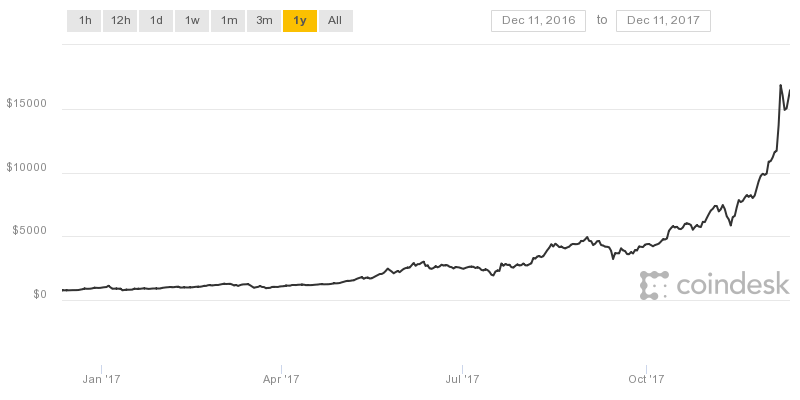
\includegraphics[width=\textwidth]{bitcoin}
\caption{Bitcoin price history from December,  2016 to December, 2017.}
\label{fig:bitcoin}
\end{figure}

		\subsubsection{Forecasting} \hspace{1cm}\\\\Time series forecasting represents the process of predicting the future values of the observed variable based on the already available data. In order to achieve that, dependencies among the available time series must be found, which then approximate the possible future values. Various methods were used over the years. They are in general divided  in two groups: linear and non-linear methods. The most significant of them will be wider presented  further in this paper. It's important to be noted that time series forecasting is just forecasting - the purpose is that the forecast is as close as possible to the future value, but there is no warranty for that. Generally applies that the deviation of the forecast increases with his time distance.\\\\ 

Time series could be not-stationary (volatile) or stationary. In other words - to have higher or lower degree of stationarity. The distribution of the stationary one depends much more on a long term trend while the distribution of the not-stationary one - on occasional events. Example for an extremely stationary time series is the coin flipping over time, example for an extremely volatile one - the bitcoin price. Because of his characteristics the volatile time series is much harder to predict. His wide spread and importance led to the development of more complex (non-linear) methods for doing that. Those methods include and are based on some machine learning techniques like e.g. bagging and boosting and also on key machine learning tools like artificial neural networks. Time series forecasting is one of the classic and at the same time very important areas of the machine learning.
	\subsection{Origins and related topics}
		\subsubsection{Machine Learning}\hspace{1cm}\\\\ 
In the recent years, as many useful applications of machine learning have been developed and have become part of our everyday life, his significance increased. We hear more and more often the term on the news or read about it on the Internet. In many cases machine learning is used as a synonym for artificial intelligence (AI), which is incorrect. AI is field of computer science, which is studying and  applying approaches for making computers being able to execute cognitive tasks. Machine learning is one of those approaches and it's by far the most successful (widely used, with the most applications) one of them. His subject is the studying and the computer modelling of learning processes.\cite{AIvsML}\cite{Michalski1983}. \\\\ One common way to create a new machine learning process is to research the human learning mechanisms, to adapt them and then accordingly to simulate them  with algorithms. The artificial neural networks (commonly utilized machine learning tool) are example for that and they will be discussed thoroughly further in the paper. It is  restrictive to believe that the learning patterns that come from the nature are the only possible way for acquiring knowledge. Reserchers also try to manifacture their own ones. By doing this main criteria are the methods'  generality and performance rather than their psychological explanation\cite{Michalski1983}.
\\\\				
		 \paragraph{Decision trees}
		 \paragraph{Artificial Neural Networks}
		 \paragraph{Ensemble Techniques}
		\subsubsection{General time series forecasting methods}
\section{Arbitrated Ensemble for Time Series Forecasting}
\subsection{General explanation}
\subsection{Learning Basic-Level Models}
\subsection{Learning Meta-Level Models}
\subsection{Predicting the next time serie}
\subsection{Performance comparison with general time series forecasting methods}

\section{Conclusion and Outlook}

\subsubsection*{Acknowledgments}

\cite{VtorCerqueira2017} In the bibliography

%%%%%%%%%%%%%%%%%%%%%%%%%%%%%%%%%%%%%%%%%%%%%%%%%%%%%%%%%%%%%%%%%%%%%%%%%%%%%%%
\bibliographystyle{splncs03}
\bibliography{paper}

%%%%%%%%%%%%%%%%%%%%%%%%%%%%%%%%%%%%%%%%%%%%%%%%%%%%%%%%%%%%%%%%%%%%%%%%%%%%%%%

\end{document}
